\documentclass{beamer}
\usepackage[utf8]{inputenc}
\usepackage{amsmath}
\usepackage{ragged2e}

\usetheme{Madrid}
\usecolortheme{default}
\justifying

%------------------------------------------------------------
%This block of code defines the information to appear in the
%Title page
%Information to be included in the title page:
\title[Radiobiological Models] %optional
{Introduction to Radiobiological Models}

\subtitle{A short story}

\author[Souvik Das] % (optional)
{
\includegraphics[height=2cm]{Tata_Memorial_Center_logo.jpg} \\ Souvik Das}
\institute[] % (optional)
{
  Resisdent Medical Physicist\\
  Tata Memorial Hospital, Mumbai
}

\date[\today] % (optional)


%End of title page configuration block
%------------------------------------------------------------



%------------------------------------------------------------
%The next block of commands puts the table of contents at the 
%beginning of each section and highlights the current section:

\AtBeginSection[]
{
  \begin{frame}
    \frametitle{Table of Contents}
    \tableofcontents[currentsection]
  \end{frame}
}
%------------------------------------------------------------


\begin{document}

%The next statement creates the title page.
\frame{\titlepage}


%---------------------------------------------------------
%This block of code is for the table of contents after
%the title page
\begin{frame}
\frametitle{Table of Contents}
\setcounter{tocdepth}{2}
\tableofcontents[]
\end{frame}
%---------------------------------------------------------


\section{Linear Quadratic (LQ) Model}

\begin{frame}
  \frametitle{Target theory}


\begin{itemize}
 \item<1-> The target of radiation for the purpose of therapy is the \textbf{DNA}.
 \item<2-> Post-irradiation \textbf{cell survival} as a function of radiation dose can be \textbf{biophysically modeled} in several different ways.
 \item<3-> \textbf{Poisson statistics} are used for the basis for survival equations.

\end{itemize}
\end{frame}



\begin{frame}
  \frametitle{Mathematical Modeling}
  \framesubtitle{Poisson Statistics}
  \begin{figure}[H]
    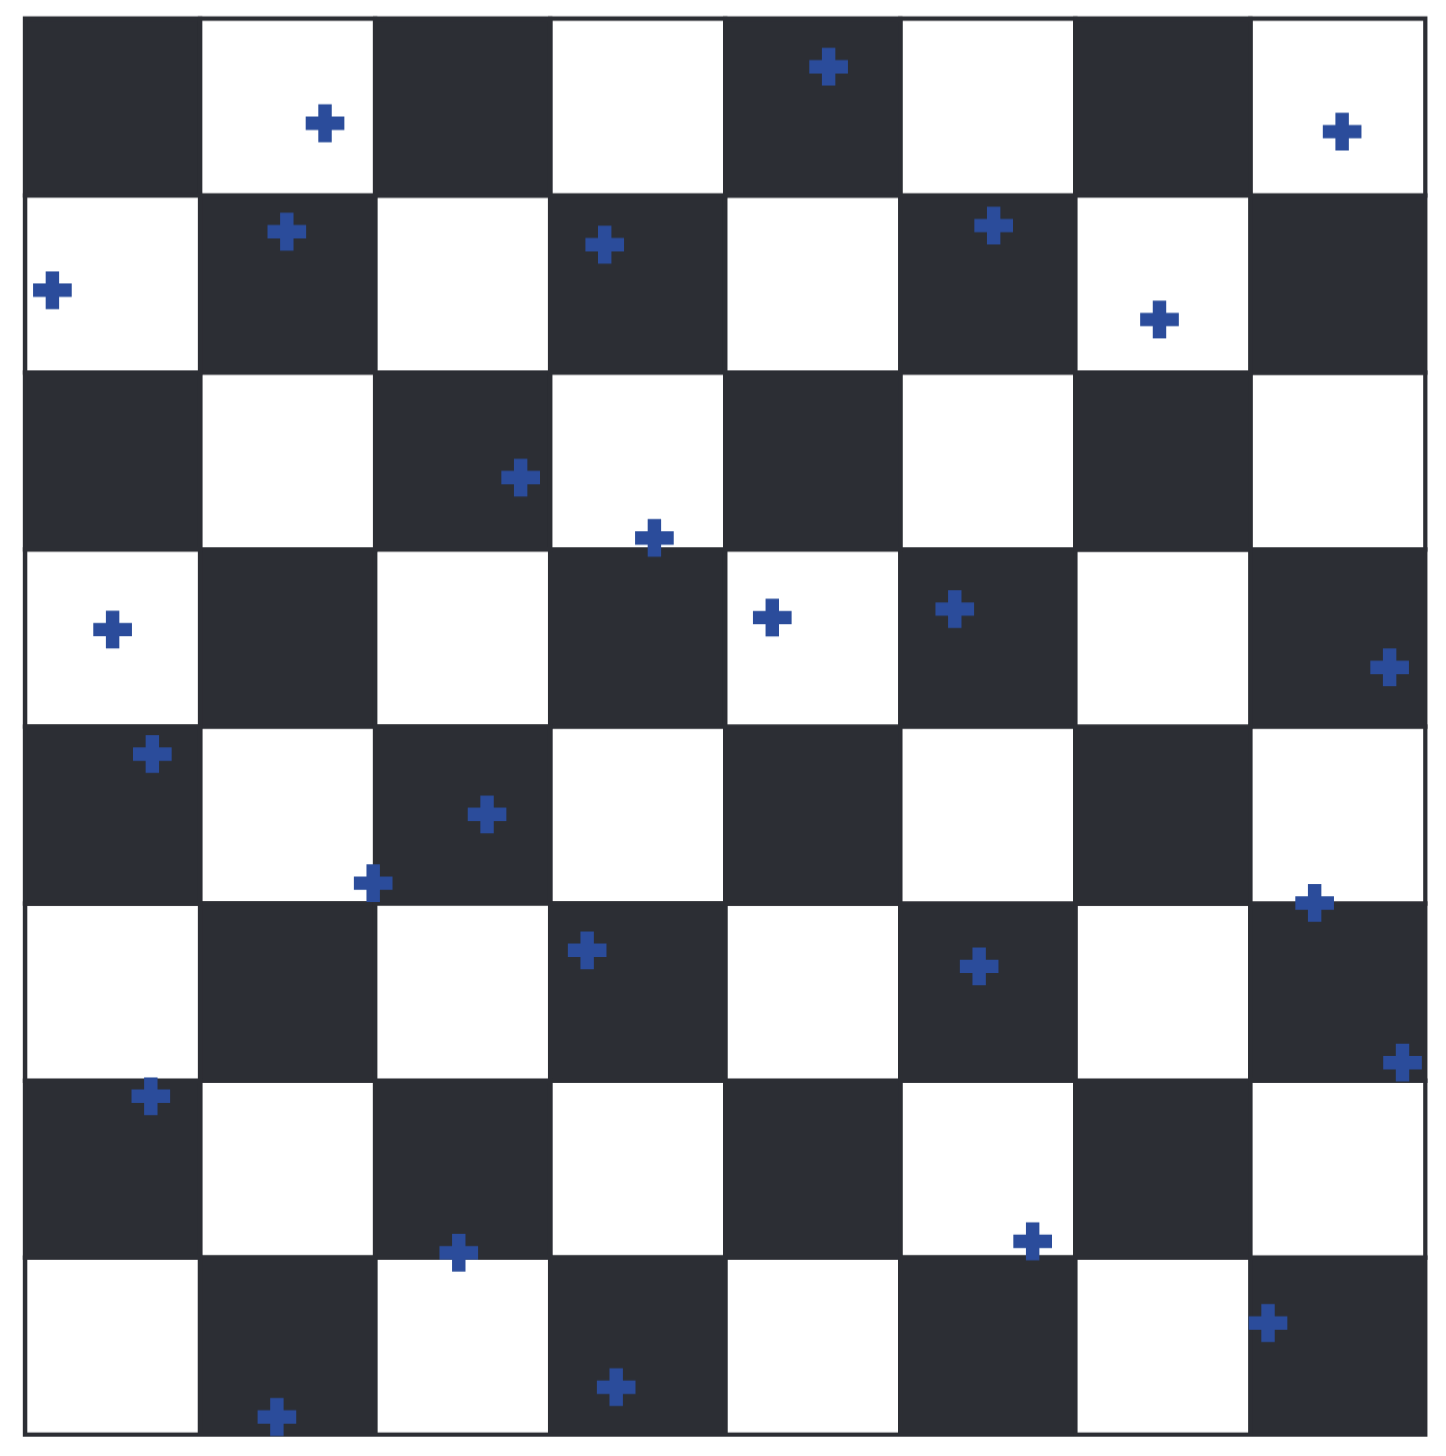
\includegraphics[width=0.3\textwidth]{ChessBoard.png}
    \caption{If it rains on a chessboard, and an average of $x$ drops hits each square,  How many squares are dry?}
  \end{figure}

  \begin{itemize}
    \item <2-> Poisson statistics describe a large number of random events happening to a  large number of subjects, averaging out to a small number of events per subject.
  \end{itemize}
\end{frame}

\begin{frame}
  \frametitle{Mathematical Modeling}
  \framesubtitle{Poisson Statistics}
  \begin{itemize}
    \item <1-> If $x$ is the average number of drops per square, then the probability of a square being hit by $k$ drops is given by:
      $$P(k) = \frac{x^k e^{-x}}{k!}$$
    \item <2-> The probability of a square being dry is given by:
      $$P(0) = e^{-x}$$
    \item <3-> The probability of a square being wet is given by:
  
      $$P(\text{wet}) = 1 - e^{-x}$$
  \end{itemize}
\end{frame}




\begin{frame}
  \frametitle{Poisson Distribution}
  \framesubtitle{Cell Survival}
  \begin{itemize}
    \item <1-> The Poisson model is used for surviving fraction (\textbf{SF}) of cells:
    \begin{itemize}
      \item <2-> At an average of $x$ lethal hits per cell:
        \begin{itemize}
          \item<3-> $e^{-x}$ cells survive (no hits).
          \item <4->$1 - e^{-x}$ cells die (at least 1 hit).
        \end{itemize}
      \item <5-> Based on this equation,
        \begin{itemize}
          \item <6-> 1 hit kills 63\% of cells. SF = 0.37
          \item <7-> 2 hits kills 86\% of cells. SF = 0.14
          \item <8-> 3 hits kills 95\% of cells. SF = 0.05
          \item <9-> 4 hits kills 98\% of cells. SF = 0.02
          \item <10-> 5 hits kills 99\% of cells. SF = 0.01
        \end{itemize}
        \begin{block}{Note}<11->
          $D_0$ is defined as the radiation dose resulting in 37\% survival. This is assumed  to be equal to the radiation dose necessary to cause one \textbf{lethal} hit per cell.
        \end{block}
    \end{itemize}
  \end{itemize}
\end{frame}


\begin{frame}
  \frametitle{Poisson Distribution}
  \framesubtitle{Tumor Control Probability (TCP)}
  \begin{itemize}
    \item <1-> The Poisson model is used for Tumor Control Probability (\textbf{TCP}) of cells:
    \begin{itemize}
      \item <2-> At an average of $x$ surviving tumor cells per patient:
        \begin{itemize}
          \item<3-> $e^{-x}$ cells survive (no hits).
          \item <4->$1 - e^{-x}$ cells die (at least 1 hit).
        \end{itemize}
      \item <5-> Based on this equation,
        \begin{itemize}
          \item <6-> 1 tumor cell per pt.: TCP = 0.37
          \item <7-> 2 tumor cell per pt.: TCP = 0.14
          \item <8-> 3 tumor cells per pt.: TCP = 0.05
          \item <9-> 4 tumor cells per pt.: TCP = 0.02
          \item <10-> 5 tumor cells per pt.: TCP = 0.01
        \end{itemize}
        \begin{block}{Note}<11->
          To achieve a certain TCP, you should aim for a tumor cell  survival of (1 - TCP).
        \end{block}
    \end{itemize}
  \end{itemize}

\end{frame}


\begin{frame}
  \frametitle{Target theory}
  \framesubtitle{Single-Target, Single-Hit Model}
  \begin{itemize}
    \item <1-> It assumes that each cell has a \textbf{single critical target}, and that a single hit to this target is sufficient to cause cell death.
    \item <2-> The survival fraction (SF) is given by:
      $$SF = e^{-D/D_0}$$
      where $D$ is the dose and $D_0$ is the dose required to reduce the surviving fraction to 37\%.
    \item <3-> This type of survival curve is seen for mammalian cells which are irradiated  with \textbf{high LET} radiation such as alpha particles or carbon ions; very \textbf{radiation-sensitive} cells like lymphocytes and bone marrow cells; cells that have major defects in DNA doublestrand break repair; are synchronized in M phase; and for cells that have DNA double-strand break repair inhibited by chemical or gene knockdown.
  \end{itemize}
\end{frame}


\begin{frame}
  \frametitle{Target theory}
  \framesubtitle{Multitarget, Single-Hit Model}
  \begin{itemize}
    \item <1-> This model assumes that each cell has multiple independent targets, all of which  must be hit to kill the cell.
    \item <2-> For a single dose D, the survival fraction (SF) is given by:
      $$SF = 1 - (1 - e^{-D/D_0})^n$$
      where $D$ is the dose, $D_0$ is the dose required to reduce the surviving fraction to 37\%, and $n$ is the number of targets.
    \item <3-> This type of survival curve is seen for mammalian cells which are irradiated with \textbf{low LET} radiation such as X-rays or gamma rays; cells that are \textbf{radiation-resistant} like fibroblasts and epithelial cells; cells that have a normal DNA double-strand break repair; and for cells that are synchronized in G1 or S phase.
  \end{itemize}
\end{frame}



\begin{frame}
  \frametitle{Target theory}
  \framesubtitle{Multitarget, Single-Hit Model}
  \begin{figure}[H]
    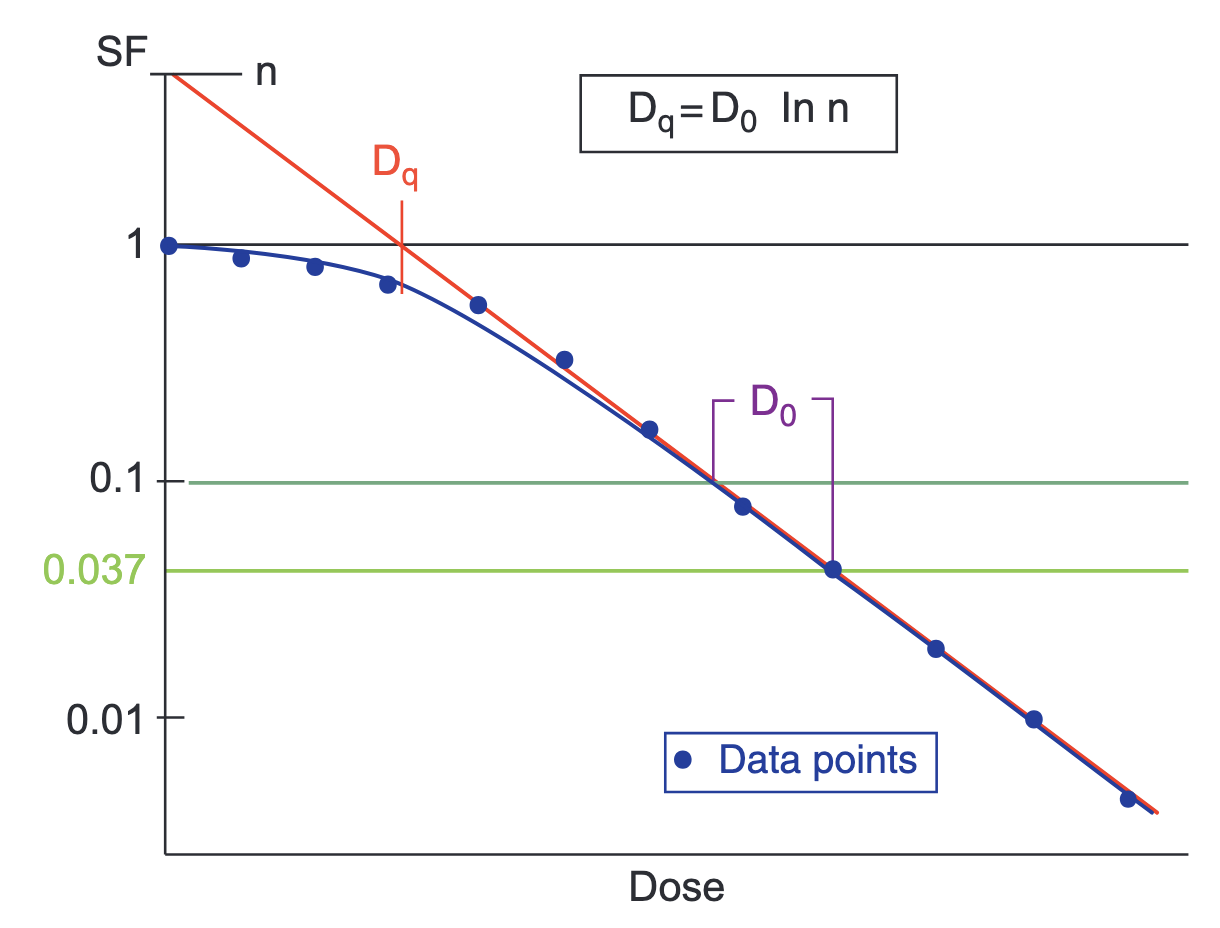
\includegraphics[width=0.6\textwidth]{CellServivalCurve.png}
    \caption{The single-hit, multitarget survival curve. Notice that it is curved at low doses and straight (e.g., survival is an exponential function of dose) at high doses. This allows you to calculate $D_0$ by taking measurements in the high-dose region}
  \end{figure}
\end{frame}



\begin{frame}
  \frametitle{Target theory}
  \framesubtitle{Multitarget, Single-Hit Model}
  \begin{itemize}
    \item<1-> The high-dose portion of the curve is actually a straight line:
    \begin{itemize}
      \item<2-> $D_0$ is defined as the additional dose required to reduce surviving fraction to  37\% of what it was before.
      \begin{alertblock}{Important to note}<3->
        Do not measure $D_0$ at SF = 0.37 if the survival curve has a shoulder. Remember that $D_0$ applies to the high-dose portion of the curve in that case! Instead, measure the difference in dose between SF = 0.1 and SF = 0.037.
      \end{alertblock}
      \item<4-> $D_0$ is a measure of the cell’s inherent radiation sensitivity. Most $D_0$ values are somewhere around 1 Gy.
      \item<5-> $D_{10}$ = $2.3 \times D_0$ = a dose that will reduce surviving fraction by tenfold (i.e., from  SF = 0.1 to SF = 0.01).
    \end{itemize}
\item<6-> The low-dose portion of the curve is known as the “shoulder”:
    \begin{itemize}
      \item<7-> $D_q$ tells you how wide the shoulder is.
      \item <8->$D_q$ is a measure of the cell's repair capacity. More repair means a larger $D_q$  and a larger shoulder
    \end{itemize}
  \end{itemize}
\end{frame}



\begin{frame}
  \frametitle{Single-Hit, Multitarget Model}
  \framesubtitle{Advantages and Disadvantages}
  

\end{frame}

\section{Nominal Standard Dose (NSD)}
\section{Cumulative Radiation Effect (CRE)}
\section{Time-Dose-Fractionation (TDF)}
\section{Practical Applications}


\end{document}